\section{Simulations}
\label{sec:simulations}
Figure \ref{fig:strongARM_out} shows the output of the stongARM latch for alternating data at the input for \unit[6]{UI}. For the simulation a data pattern of 11001100 was feed into the input of the receiver. As we have two slices with half-rate clocking this results in alternating data for one of the slices. To degenerate the signal and take the limited bandwith of the channel into account a RC circuit was used at the receiver input resulting in the \textit{in+} and \textit{in-} signals. The \textit{set} and \textit{reset} signals are the direct outputs of the strongARM circuit and the \textit{RS\_out} signal is one of the RS-FlipFlop outputs.

The frequency response of the variable offset amplifier (VOA) is shown in figure \ref{fig:voa_freq} and its ac noise response is drawn in figure \ref{fig:voa_noise}.

\begin{figure}[H]
  \centering
  {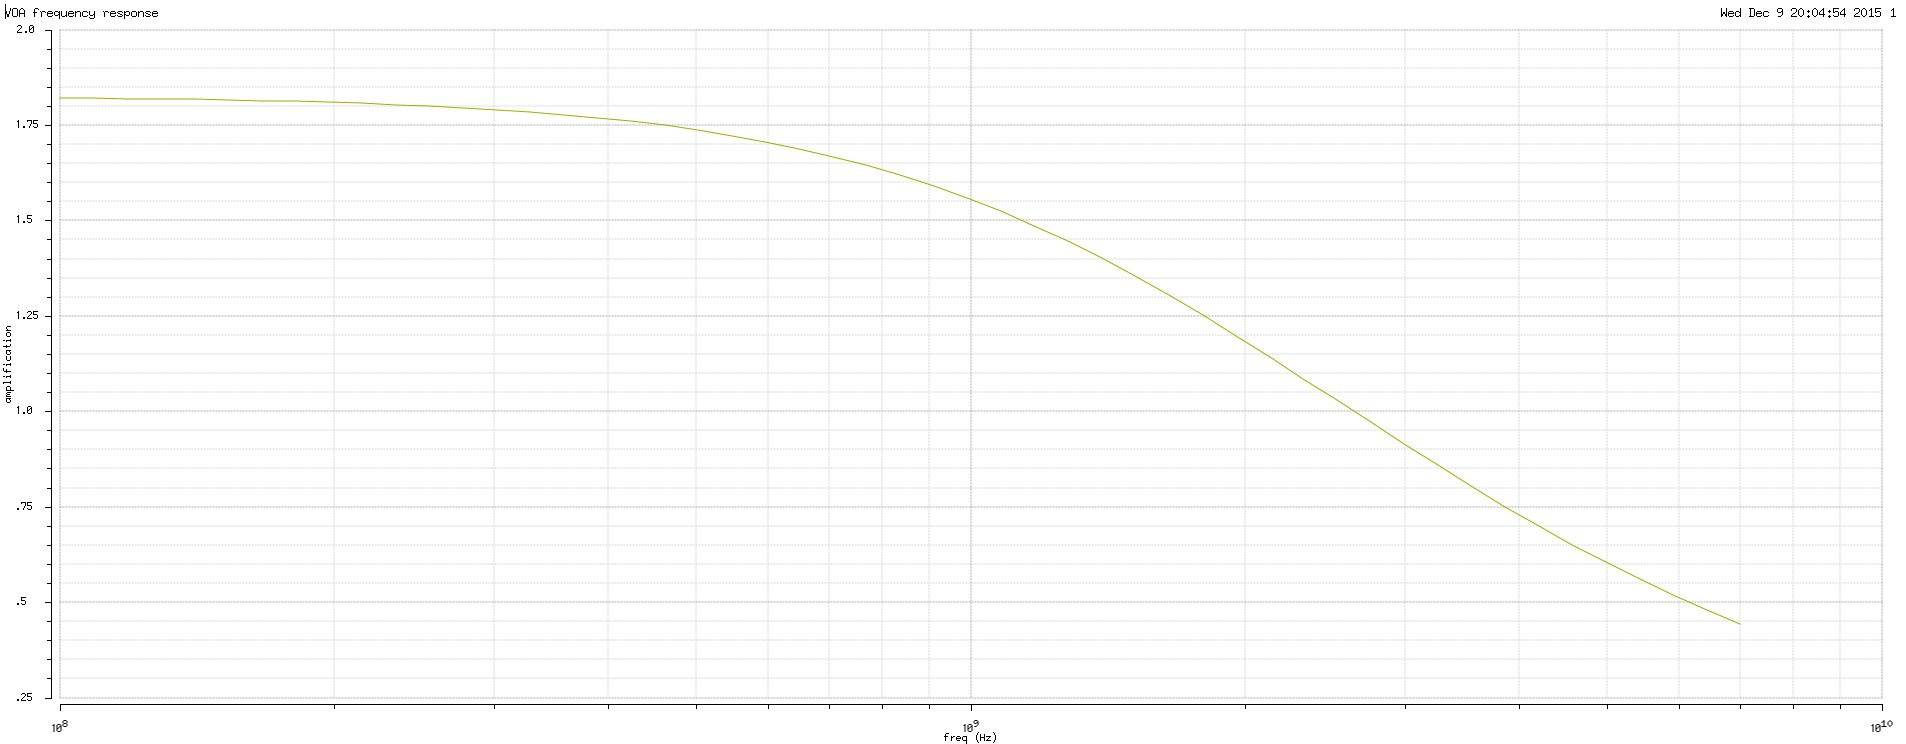
\includegraphics[scale=0.35]{img/voa_freq.jpg}}
  \caption{VOA frequency response}
  \label{fig:voa_freq}
\end{figure}

\begin{figure}[H]
  \centering
  {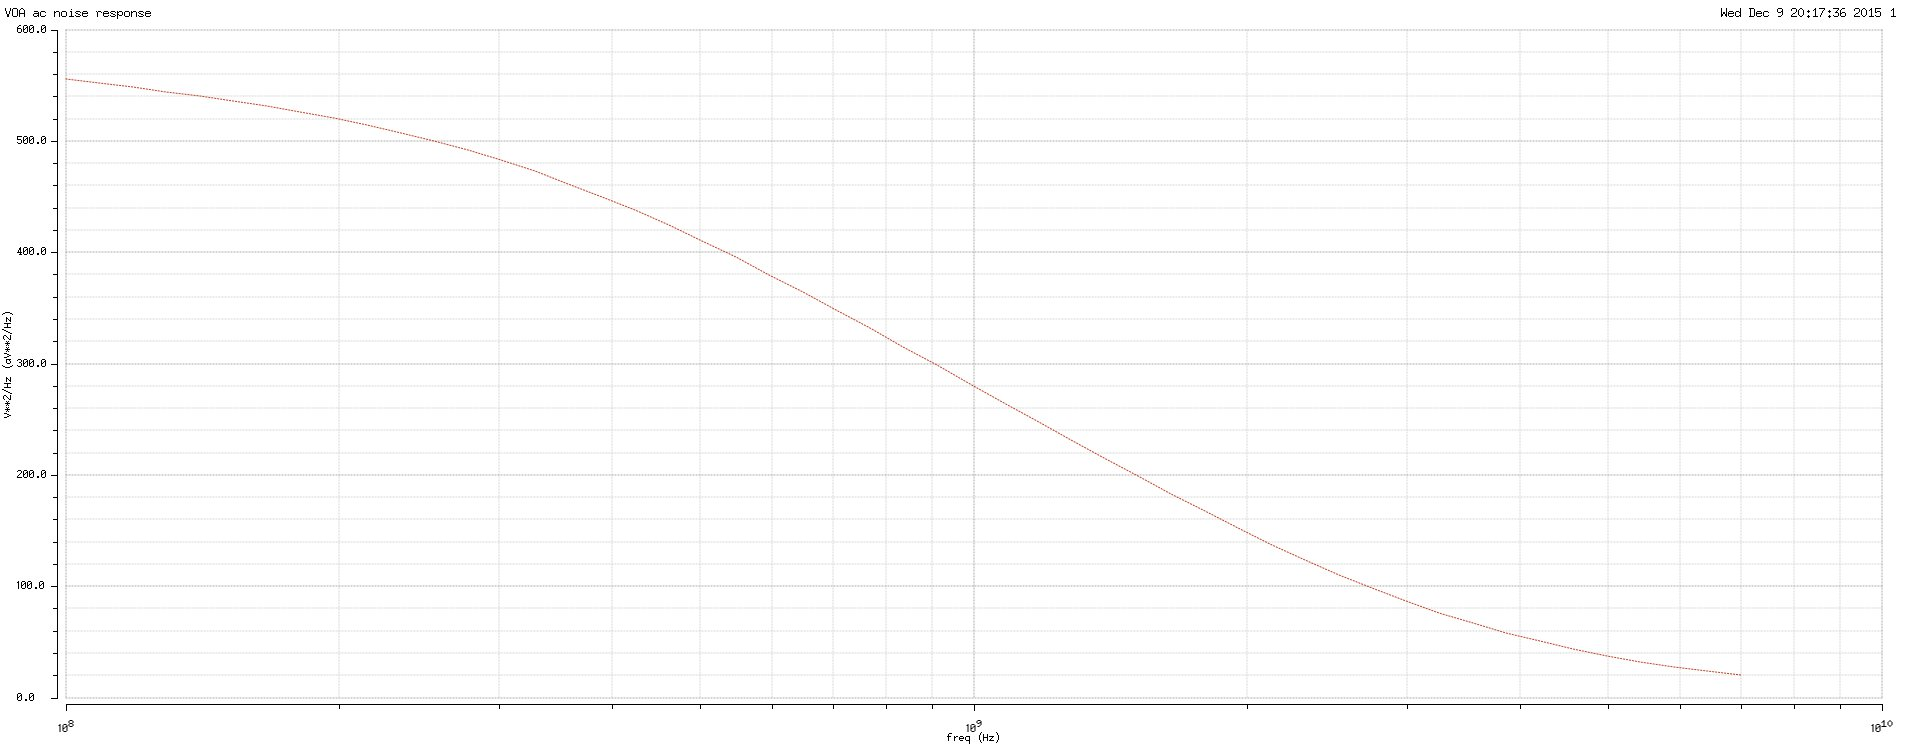
\includegraphics[scale=0.35]{img/voa_noise.jpg}}
  \caption{VOA ac noise response}
  \label{fig:voa_noise}
\end{figure}

\begin{figure}[H]
  \centering
  {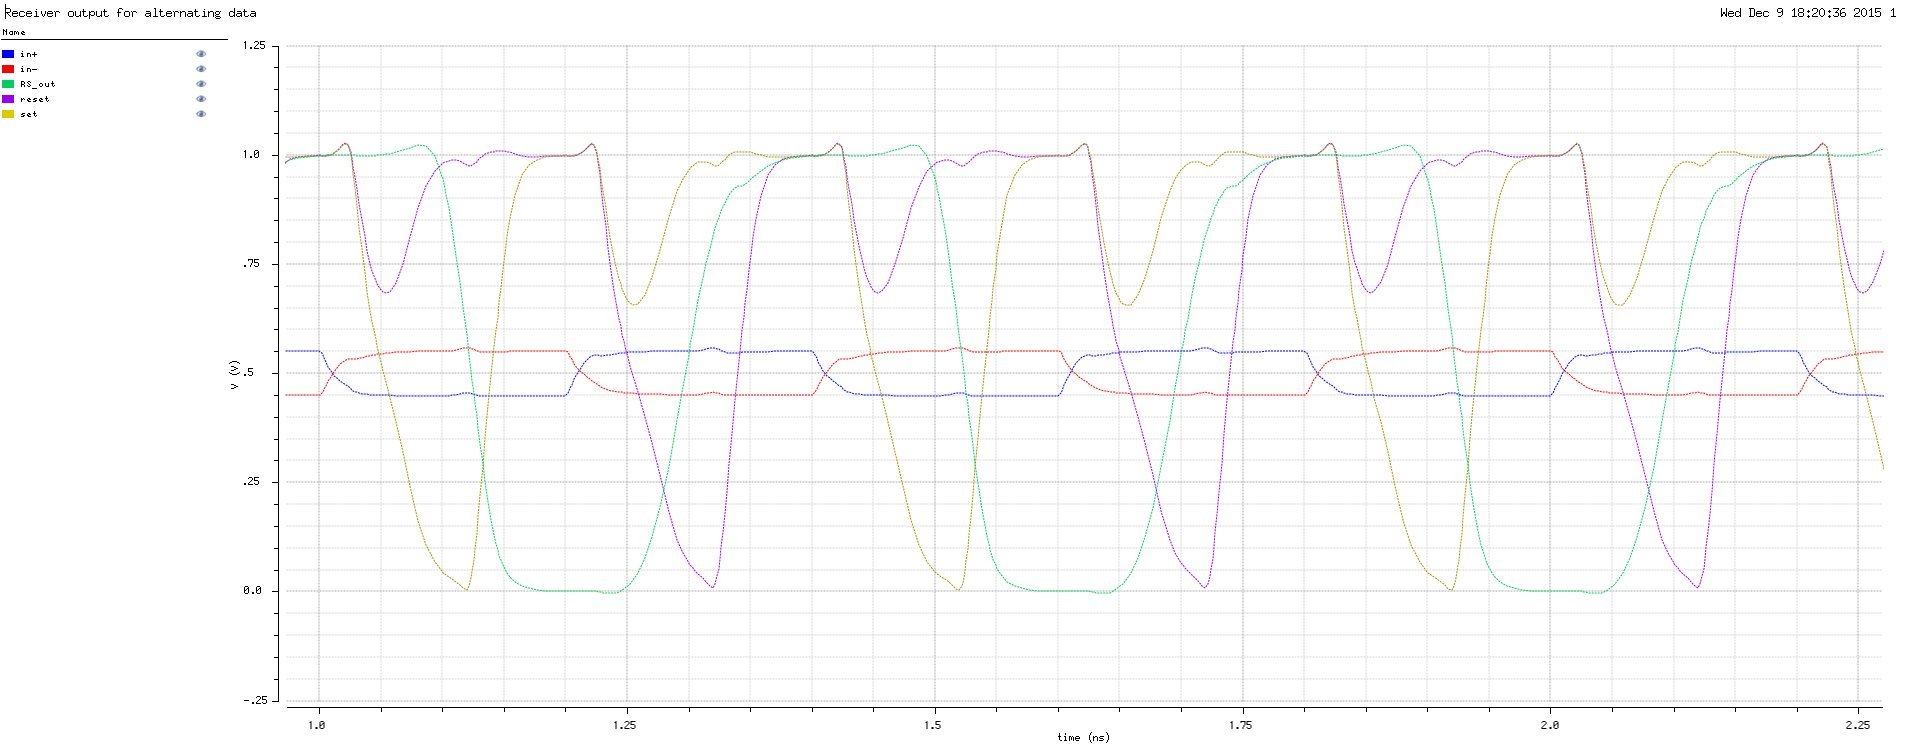
\includegraphics[angle=90, scale=0.45]{img/output_alt_trans.jpg}}
  \caption{Transient waveform for alternating data at the output of the strongARM latch}
  \label{fig:strongARM_out}
\end{figure}

In figure \ref{fig:rx_slice_pdf_cdf} the CDF and PDF for a single receiver slice are shown. As hysteresis was greater than the noise (resulting in a step function as CDF) the simulation was done with scaling transient noise by a factor of four. Therefore to get the right values for the noise the x-axis has to be divided by 4. The simulation should be run a bit longer to see the full CDF/PDF.

\begin{figure}[H]
  \centering
  \subfigure[CDF]
  {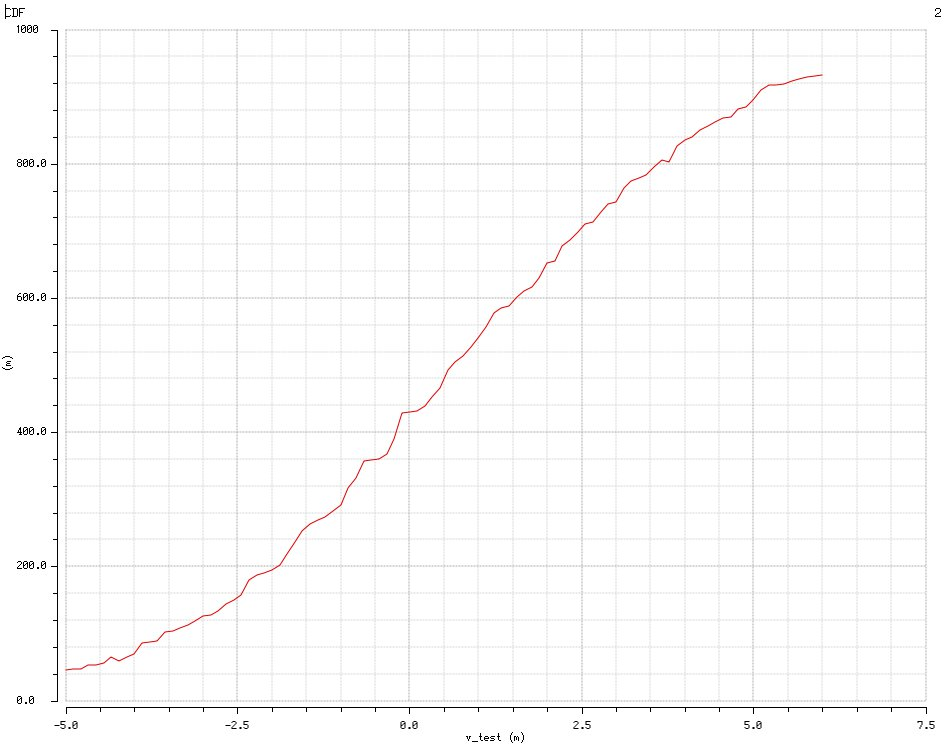
\includegraphics[scale=0.5]{img/rx_slice_cdf.jpg}}
  %\subfigure[PDF]
  %{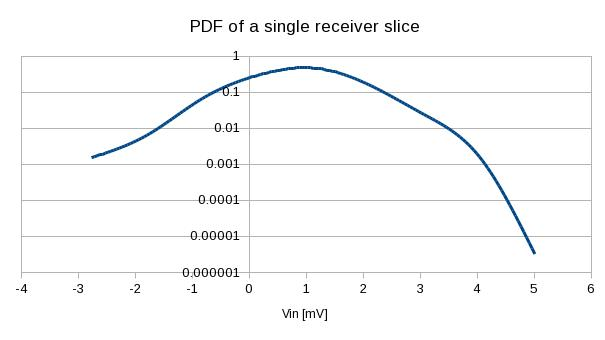
\includegraphics[scale=0.5]{img/rx_slice_pdf.jpg}}
  \caption{Input referred transient noise for a single RX slice}
  \label{fig:rx_slice_pdf_cdf}
\end{figure}

The eye diagram for \unit[10.000]{UI} at the receiver output is given in figure \ref{fig:rx_out_eye}. The outputs of both receiver slices are shown in the eye diagram.

\begin{figure}[H]
  \centering
  {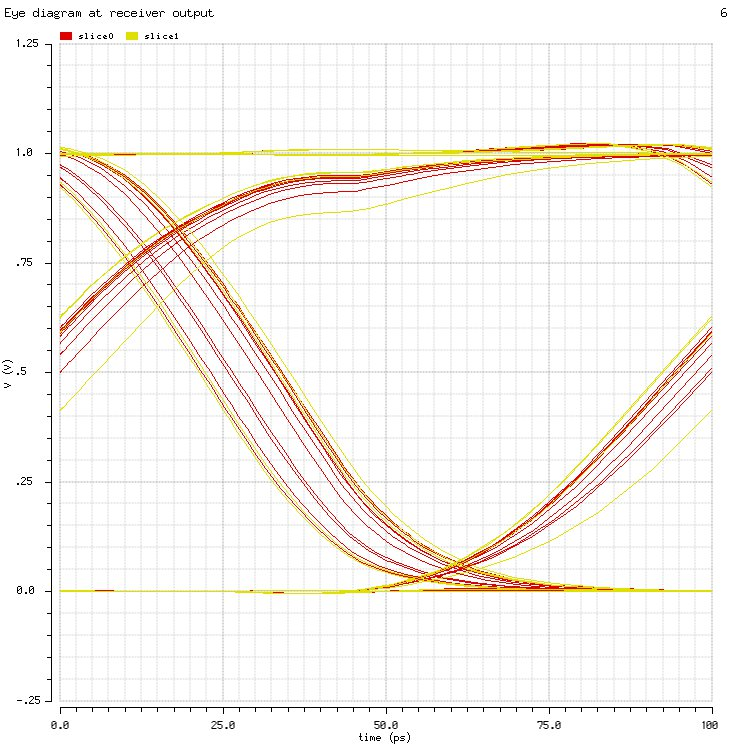
\includegraphics[scale=0.8]{img/rx_out_eye.jpg}}
  \caption{Eye diagram at the receiver output for \unit[10.000]{UI}}
  \label{fig:rx_out_eye}
\end{figure}